% Created by tikzDevice version 0.12
% !TEX encoding = UTF-8 Unicode
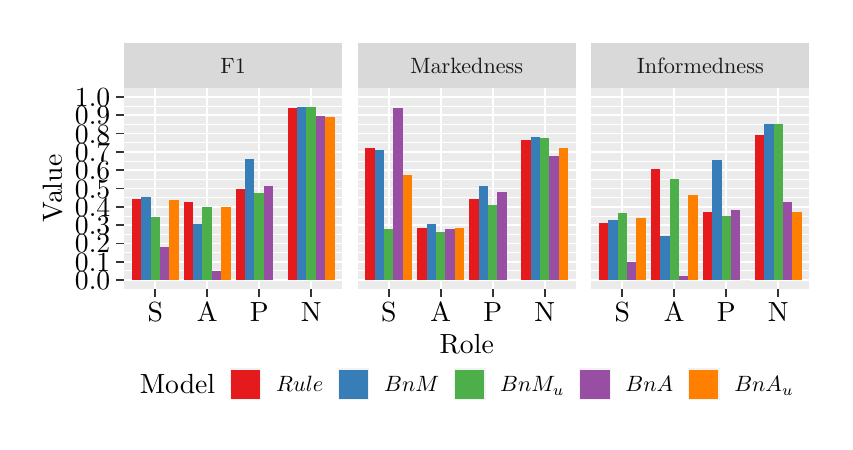
\begin{tikzpicture}[x=1pt,y=1pt]
\definecolor{fillColor}{RGB}{255,255,255}
\path[use as bounding box,fill=fillColor,fill opacity=0.00] (0,0) rectangle (288.00,142.39);
\begin{scope}
\path[clip] (  0.00,  0.00) rectangle (288.00,142.39);
\definecolor{drawColor}{RGB}{255,255,255}
\definecolor{fillColor}{RGB}{255,255,255}

\path[draw=drawColor,line width= 0.6pt,line join=round,line cap=round,fill=fillColor] (  0.00,  0.00) rectangle (288.00,142.39);
\end{scope}
\begin{scope}
\path[clip] ( 34.81, 47.91) rectangle (113.70,120.63);
\definecolor{fillColor}{gray}{0.92}

\path[fill=fillColor] ( 34.81, 47.91) rectangle (113.70,120.63);
\definecolor{drawColor}{RGB}{255,255,255}

\path[draw=drawColor,line width= 0.3pt,line join=round] ( 34.81, 54.52) --
	(113.70, 54.52);

\path[draw=drawColor,line width= 0.3pt,line join=round] ( 34.81, 61.13) --
	(113.70, 61.13);

\path[draw=drawColor,line width= 0.3pt,line join=round] ( 34.81, 67.74) --
	(113.70, 67.74);

\path[draw=drawColor,line width= 0.3pt,line join=round] ( 34.81, 74.35) --
	(113.70, 74.35);

\path[draw=drawColor,line width= 0.3pt,line join=round] ( 34.81, 80.96) --
	(113.70, 80.96);

\path[draw=drawColor,line width= 0.3pt,line join=round] ( 34.81, 87.58) --
	(113.70, 87.58);

\path[draw=drawColor,line width= 0.3pt,line join=round] ( 34.81, 94.19) --
	(113.70, 94.19);

\path[draw=drawColor,line width= 0.3pt,line join=round] ( 34.81,100.80) --
	(113.70,100.80);

\path[draw=drawColor,line width= 0.3pt,line join=round] ( 34.81,107.41) --
	(113.70,107.41);

\path[draw=drawColor,line width= 0.3pt,line join=round] ( 34.81,114.02) --
	(113.70,114.02);

\path[draw=drawColor,line width= 0.6pt,line join=round] ( 34.81, 51.21) --
	(113.70, 51.21);

\path[draw=drawColor,line width= 0.6pt,line join=round] ( 34.81, 57.82) --
	(113.70, 57.82);

\path[draw=drawColor,line width= 0.6pt,line join=round] ( 34.81, 64.44) --
	(113.70, 64.44);

\path[draw=drawColor,line width= 0.6pt,line join=round] ( 34.81, 71.05) --
	(113.70, 71.05);

\path[draw=drawColor,line width= 0.6pt,line join=round] ( 34.81, 77.66) --
	(113.70, 77.66);

\path[draw=drawColor,line width= 0.6pt,line join=round] ( 34.81, 84.27) --
	(113.70, 84.27);

\path[draw=drawColor,line width= 0.6pt,line join=round] ( 34.81, 90.88) --
	(113.70, 90.88);

\path[draw=drawColor,line width= 0.6pt,line join=round] ( 34.81, 97.49) --
	(113.70, 97.49);

\path[draw=drawColor,line width= 0.6pt,line join=round] ( 34.81,104.10) --
	(113.70,104.10);

\path[draw=drawColor,line width= 0.6pt,line join=round] ( 34.81,110.72) --
	(113.70,110.72);

\path[draw=drawColor,line width= 0.6pt,line join=round] ( 34.81,117.33) --
	(113.70,117.33);

\path[draw=drawColor,line width= 0.6pt,line join=round] ( 46.08, 47.91) --
	( 46.08,120.63);

\path[draw=drawColor,line width= 0.6pt,line join=round] ( 64.86, 47.91) --
	( 64.86,120.63);

\path[draw=drawColor,line width= 0.6pt,line join=round] ( 83.65, 47.91) --
	( 83.65,120.63);

\path[draw=drawColor,line width= 0.6pt,line join=round] (102.43, 47.91) --
	(102.43,120.63);
\definecolor{fillColor}{RGB}{255,127,0}

\path[fill=fillColor] ( 51.15, 51.21) rectangle ( 54.53, 80.29);
\definecolor{fillColor}{RGB}{152,78,163}

\path[fill=fillColor] ( 47.77, 51.21) rectangle ( 51.15, 63.24);
\definecolor{fillColor}{RGB}{77,175,74}

\path[fill=fillColor] ( 44.39, 51.21) rectangle ( 47.77, 73.82);
\definecolor{fillColor}{RGB}{55,126,184}

\path[fill=fillColor] ( 41.00, 51.21) rectangle ( 44.39, 81.24);
\definecolor{fillColor}{RGB}{228,26,28}

\path[fill=fillColor] ( 37.62, 51.21) rectangle ( 41.00, 80.51);
\definecolor{fillColor}{RGB}{255,127,0}

\path[fill=fillColor] ( 69.93, 51.21) rectangle ( 73.32, 77.45);
\definecolor{fillColor}{RGB}{152,78,163}

\path[fill=fillColor] ( 66.55, 51.21) rectangle ( 69.93, 54.40);
\definecolor{fillColor}{RGB}{77,175,74}

\path[fill=fillColor] ( 63.17, 51.21) rectangle ( 66.55, 77.52);
\definecolor{fillColor}{RGB}{55,126,184}

\path[fill=fillColor] ( 59.79, 51.21) rectangle ( 63.17, 71.37);
\definecolor{fillColor}{RGB}{228,26,28}

\path[fill=fillColor] ( 56.41, 51.21) rectangle ( 59.79, 79.35);
\definecolor{fillColor}{RGB}{152,78,163}

\path[fill=fillColor] ( 85.34, 51.21) rectangle ( 88.72, 85.19);
\definecolor{fillColor}{RGB}{77,175,74}

\path[fill=fillColor] ( 81.96, 51.21) rectangle ( 85.34, 82.79);
\definecolor{fillColor}{RGB}{55,126,184}

\path[fill=fillColor] ( 78.58, 51.21) rectangle ( 81.96, 94.81);
\definecolor{fillColor}{RGB}{228,26,28}

\path[fill=fillColor] ( 75.19, 51.21) rectangle ( 78.58, 84.11);
\definecolor{fillColor}{RGB}{255,127,0}

\path[fill=fillColor] (107.50, 51.21) rectangle (110.89,110.09);
\definecolor{fillColor}{RGB}{152,78,163}

\path[fill=fillColor] (104.12, 51.21) rectangle (107.50,110.31);
\definecolor{fillColor}{RGB}{77,175,74}

\path[fill=fillColor] (100.74, 51.21) rectangle (104.12,113.62);
\definecolor{fillColor}{RGB}{55,126,184}

\path[fill=fillColor] ( 97.36, 51.21) rectangle (100.74,113.70);
\definecolor{fillColor}{RGB}{228,26,28}

\path[fill=fillColor] ( 93.98, 51.21) rectangle ( 97.36,113.24);
\end{scope}
\begin{scope}
\path[clip] (119.20, 47.91) rectangle (198.10,120.63);
\definecolor{fillColor}{gray}{0.92}

\path[fill=fillColor] (119.20, 47.91) rectangle (198.10,120.63);
\definecolor{drawColor}{RGB}{255,255,255}

\path[draw=drawColor,line width= 0.3pt,line join=round] (119.20, 54.52) --
	(198.10, 54.52);

\path[draw=drawColor,line width= 0.3pt,line join=round] (119.20, 61.13) --
	(198.10, 61.13);

\path[draw=drawColor,line width= 0.3pt,line join=round] (119.20, 67.74) --
	(198.10, 67.74);

\path[draw=drawColor,line width= 0.3pt,line join=round] (119.20, 74.35) --
	(198.10, 74.35);

\path[draw=drawColor,line width= 0.3pt,line join=round] (119.20, 80.96) --
	(198.10, 80.96);

\path[draw=drawColor,line width= 0.3pt,line join=round] (119.20, 87.58) --
	(198.10, 87.58);

\path[draw=drawColor,line width= 0.3pt,line join=round] (119.20, 94.19) --
	(198.10, 94.19);

\path[draw=drawColor,line width= 0.3pt,line join=round] (119.20,100.80) --
	(198.10,100.80);

\path[draw=drawColor,line width= 0.3pt,line join=round] (119.20,107.41) --
	(198.10,107.41);

\path[draw=drawColor,line width= 0.3pt,line join=round] (119.20,114.02) --
	(198.10,114.02);

\path[draw=drawColor,line width= 0.6pt,line join=round] (119.20, 51.21) --
	(198.10, 51.21);

\path[draw=drawColor,line width= 0.6pt,line join=round] (119.20, 57.82) --
	(198.10, 57.82);

\path[draw=drawColor,line width= 0.6pt,line join=round] (119.20, 64.44) --
	(198.10, 64.44);

\path[draw=drawColor,line width= 0.6pt,line join=round] (119.20, 71.05) --
	(198.10, 71.05);

\path[draw=drawColor,line width= 0.6pt,line join=round] (119.20, 77.66) --
	(198.10, 77.66);

\path[draw=drawColor,line width= 0.6pt,line join=round] (119.20, 84.27) --
	(198.10, 84.27);

\path[draw=drawColor,line width= 0.6pt,line join=round] (119.20, 90.88) --
	(198.10, 90.88);

\path[draw=drawColor,line width= 0.6pt,line join=round] (119.20, 97.49) --
	(198.10, 97.49);

\path[draw=drawColor,line width= 0.6pt,line join=round] (119.20,104.10) --
	(198.10,104.10);

\path[draw=drawColor,line width= 0.6pt,line join=round] (119.20,110.72) --
	(198.10,110.72);

\path[draw=drawColor,line width= 0.6pt,line join=round] (119.20,117.33) --
	(198.10,117.33);

\path[draw=drawColor,line width= 0.6pt,line join=round] (130.48, 47.91) --
	(130.48,120.63);

\path[draw=drawColor,line width= 0.6pt,line join=round] (149.26, 47.91) --
	(149.26,120.63);

\path[draw=drawColor,line width= 0.6pt,line join=round] (168.05, 47.91) --
	(168.05,120.63);

\path[draw=drawColor,line width= 0.6pt,line join=round] (186.83, 47.91) --
	(186.83,120.63);
\definecolor{fillColor}{RGB}{255,127,0}

\path[fill=fillColor] (135.55, 51.21) rectangle (138.93, 89.11);
\definecolor{fillColor}{RGB}{152,78,163}

\path[fill=fillColor] (132.17, 51.21) rectangle (135.55,113.45);
\definecolor{fillColor}{RGB}{77,175,74}

\path[fill=fillColor] (128.78, 51.21) rectangle (132.17, 69.62);
\definecolor{fillColor}{RGB}{55,126,184}

\path[fill=fillColor] (125.40, 51.21) rectangle (128.78, 98.01);
\definecolor{fillColor}{RGB}{228,26,28}

\path[fill=fillColor] (122.02, 51.21) rectangle (125.40, 99.02);
\definecolor{fillColor}{RGB}{255,127,0}

\path[fill=fillColor] (154.33, 51.21) rectangle (157.71, 70.15);
\definecolor{fillColor}{RGB}{152,78,163}

\path[fill=fillColor] (150.95, 51.21) rectangle (154.33, 69.63);
\definecolor{fillColor}{RGB}{77,175,74}

\path[fill=fillColor] (147.57, 51.21) rectangle (150.95, 68.72);
\definecolor{fillColor}{RGB}{55,126,184}

\path[fill=fillColor] (144.19, 51.21) rectangle (147.57, 71.56);
\definecolor{fillColor}{RGB}{228,26,28}

\path[fill=fillColor] (140.81, 51.21) rectangle (144.19, 70.13);
\definecolor{fillColor}{RGB}{152,78,163}

\path[fill=fillColor] (169.74, 51.21) rectangle (173.12, 82.98);
\definecolor{fillColor}{RGB}{77,175,74}

\path[fill=fillColor] (166.35, 51.21) rectangle (169.74, 78.39);
\definecolor{fillColor}{RGB}{55,126,184}

\path[fill=fillColor] (162.97, 51.21) rectangle (166.35, 85.24);
\definecolor{fillColor}{RGB}{228,26,28}

\path[fill=fillColor] (159.59, 51.21) rectangle (162.97, 80.63);
\definecolor{fillColor}{RGB}{255,127,0}

\path[fill=fillColor] (191.90, 51.21) rectangle (195.28, 98.73);
\definecolor{fillColor}{RGB}{152,78,163}

\path[fill=fillColor] (188.52, 51.21) rectangle (191.90, 96.13);
\definecolor{fillColor}{RGB}{77,175,74}

\path[fill=fillColor] (185.14, 51.21) rectangle (188.52,102.58);
\definecolor{fillColor}{RGB}{55,126,184}

\path[fill=fillColor] (181.76, 51.21) rectangle (185.14,102.91);
\definecolor{fillColor}{RGB}{228,26,28}

\path[fill=fillColor] (178.38, 51.21) rectangle (181.76,101.77);
\end{scope}
\begin{scope}
\path[clip] (203.60, 47.91) rectangle (282.50,120.63);
\definecolor{fillColor}{gray}{0.92}

\path[fill=fillColor] (203.60, 47.91) rectangle (282.50,120.63);
\definecolor{drawColor}{RGB}{255,255,255}

\path[draw=drawColor,line width= 0.3pt,line join=round] (203.60, 54.52) --
	(282.50, 54.52);

\path[draw=drawColor,line width= 0.3pt,line join=round] (203.60, 61.13) --
	(282.50, 61.13);

\path[draw=drawColor,line width= 0.3pt,line join=round] (203.60, 67.74) --
	(282.50, 67.74);

\path[draw=drawColor,line width= 0.3pt,line join=round] (203.60, 74.35) --
	(282.50, 74.35);

\path[draw=drawColor,line width= 0.3pt,line join=round] (203.60, 80.96) --
	(282.50, 80.96);

\path[draw=drawColor,line width= 0.3pt,line join=round] (203.60, 87.58) --
	(282.50, 87.58);

\path[draw=drawColor,line width= 0.3pt,line join=round] (203.60, 94.19) --
	(282.50, 94.19);

\path[draw=drawColor,line width= 0.3pt,line join=round] (203.60,100.80) --
	(282.50,100.80);

\path[draw=drawColor,line width= 0.3pt,line join=round] (203.60,107.41) --
	(282.50,107.41);

\path[draw=drawColor,line width= 0.3pt,line join=round] (203.60,114.02) --
	(282.50,114.02);

\path[draw=drawColor,line width= 0.6pt,line join=round] (203.60, 51.21) --
	(282.50, 51.21);

\path[draw=drawColor,line width= 0.6pt,line join=round] (203.60, 57.82) --
	(282.50, 57.82);

\path[draw=drawColor,line width= 0.6pt,line join=round] (203.60, 64.44) --
	(282.50, 64.44);

\path[draw=drawColor,line width= 0.6pt,line join=round] (203.60, 71.05) --
	(282.50, 71.05);

\path[draw=drawColor,line width= 0.6pt,line join=round] (203.60, 77.66) --
	(282.50, 77.66);

\path[draw=drawColor,line width= 0.6pt,line join=round] (203.60, 84.27) --
	(282.50, 84.27);

\path[draw=drawColor,line width= 0.6pt,line join=round] (203.60, 90.88) --
	(282.50, 90.88);

\path[draw=drawColor,line width= 0.6pt,line join=round] (203.60, 97.49) --
	(282.50, 97.49);

\path[draw=drawColor,line width= 0.6pt,line join=round] (203.60,104.10) --
	(282.50,104.10);

\path[draw=drawColor,line width= 0.6pt,line join=round] (203.60,110.72) --
	(282.50,110.72);

\path[draw=drawColor,line width= 0.6pt,line join=round] (203.60,117.33) --
	(282.50,117.33);

\path[draw=drawColor,line width= 0.6pt,line join=round] (214.87, 47.91) --
	(214.87,120.63);

\path[draw=drawColor,line width= 0.6pt,line join=round] (233.66, 47.91) --
	(233.66,120.63);

\path[draw=drawColor,line width= 0.6pt,line join=round] (252.44, 47.91) --
	(252.44,120.63);

\path[draw=drawColor,line width= 0.6pt,line join=round] (271.23, 47.91) --
	(271.23,120.63);
\definecolor{fillColor}{RGB}{255,127,0}

\path[fill=fillColor] (219.95, 51.21) rectangle (223.33, 73.72);
\definecolor{fillColor}{RGB}{152,78,163}

\path[fill=fillColor] (216.56, 51.21) rectangle (219.95, 57.84);
\definecolor{fillColor}{RGB}{77,175,74}

\path[fill=fillColor] (213.18, 51.21) rectangle (216.56, 75.42);
\definecolor{fillColor}{RGB}{55,126,184}

\path[fill=fillColor] (209.80, 51.21) rectangle (213.18, 72.72);
\definecolor{fillColor}{RGB}{228,26,28}

\path[fill=fillColor] (206.42, 51.21) rectangle (209.80, 71.80);
\definecolor{fillColor}{RGB}{255,127,0}

\path[fill=fillColor] (238.73, 51.21) rectangle (242.11, 82.05);
\definecolor{fillColor}{RGB}{152,78,163}

\path[fill=fillColor] (235.35, 51.21) rectangle (238.73, 52.73);
\definecolor{fillColor}{RGB}{77,175,74}

\path[fill=fillColor] (231.97, 51.21) rectangle (235.35, 87.65);
\definecolor{fillColor}{RGB}{55,126,184}

\path[fill=fillColor] (228.59, 51.21) rectangle (231.97, 67.09);
\definecolor{fillColor}{RGB}{228,26,28}

\path[fill=fillColor] (225.20, 51.21) rectangle (228.59, 91.40);
\definecolor{fillColor}{RGB}{255,127,0}

\path[fill=fillColor] (257.52, 51.21) rectangle (260.90, 51.21);
\definecolor{fillColor}{RGB}{152,78,163}

\path[fill=fillColor] (254.13, 51.21) rectangle (257.52, 76.63);
\definecolor{fillColor}{RGB}{77,175,74}

\path[fill=fillColor] (250.75, 51.21) rectangle (254.13, 74.32);
\definecolor{fillColor}{RGB}{55,126,184}

\path[fill=fillColor] (247.37, 51.21) rectangle (250.75, 94.67);
\definecolor{fillColor}{RGB}{228,26,28}

\path[fill=fillColor] (243.99, 51.21) rectangle (247.37, 75.66);
\definecolor{fillColor}{RGB}{255,127,0}

\path[fill=fillColor] (276.30, 51.21) rectangle (279.68, 75.69);
\definecolor{fillColor}{RGB}{152,78,163}

\path[fill=fillColor] (272.92, 51.21) rectangle (276.30, 79.48);
\definecolor{fillColor}{RGB}{77,175,74}

\path[fill=fillColor] (269.54, 51.21) rectangle (272.92,107.73);
\definecolor{fillColor}{RGB}{55,126,184}

\path[fill=fillColor] (266.16, 51.21) rectangle (269.54,107.44);
\definecolor{fillColor}{RGB}{228,26,28}

\path[fill=fillColor] (262.78, 51.21) rectangle (266.16,103.66);
\end{scope}
\begin{scope}
\path[clip] ( 34.81,120.63) rectangle (113.70,136.89);
\definecolor{fillColor}{gray}{0.85}

\path[fill=fillColor] ( 34.81,120.63) rectangle (113.70,136.89);
\definecolor{drawColor}{gray}{0.10}

\node[text=drawColor,anchor=base,inner sep=0pt, outer sep=0pt, scale=  0.80] at ( 74.25,126.01) {F1};
\end{scope}
\begin{scope}
\path[clip] (119.20,120.63) rectangle (198.10,136.89);
\definecolor{fillColor}{gray}{0.85}

\path[fill=fillColor] (119.20,120.63) rectangle (198.10,136.89);
\definecolor{drawColor}{gray}{0.10}

\node[text=drawColor,anchor=base,inner sep=0pt, outer sep=0pt, scale=  0.80] at (158.65,126.01) {Markedness};
\end{scope}
\begin{scope}
\path[clip] (203.60,120.63) rectangle (282.50,136.89);
\definecolor{fillColor}{gray}{0.85}

\path[fill=fillColor] (203.60,120.63) rectangle (282.50,136.89);
\definecolor{drawColor}{gray}{0.10}

\node[text=drawColor,anchor=base,inner sep=0pt, outer sep=0pt, scale=  0.80] at (243.05,126.01) {Informedness};
\end{scope}
\begin{scope}
\path[clip] (  0.00,  0.00) rectangle (288.00,142.39);
\definecolor{drawColor}{gray}{0.20}

\path[draw=drawColor,line width= 0.6pt,line join=round] ( 46.08, 45.16) --
	( 46.08, 47.91);

\path[draw=drawColor,line width= 0.6pt,line join=round] ( 64.86, 45.16) --
	( 64.86, 47.91);

\path[draw=drawColor,line width= 0.6pt,line join=round] ( 83.65, 45.16) --
	( 83.65, 47.91);

\path[draw=drawColor,line width= 0.6pt,line join=round] (102.43, 45.16) --
	(102.43, 47.91);
\end{scope}
\begin{scope}
\path[clip] (  0.00,  0.00) rectangle (288.00,142.39);
\definecolor{drawColor}{RGB}{0,0,0}

\node[text=drawColor,anchor=base,inner sep=0pt, outer sep=0pt, scale=  1.00] at ( 46.08, 36.07) {S};

\node[text=drawColor,anchor=base,inner sep=0pt, outer sep=0pt, scale=  1.00] at ( 64.86, 36.07) {A};

\node[text=drawColor,anchor=base,inner sep=0pt, outer sep=0pt, scale=  1.00] at ( 83.65, 36.07) {P};

\node[text=drawColor,anchor=base,inner sep=0pt, outer sep=0pt, scale=  1.00] at (102.43, 36.07) {N};
\end{scope}
\begin{scope}
\path[clip] (  0.00,  0.00) rectangle (288.00,142.39);
\definecolor{drawColor}{gray}{0.20}

\path[draw=drawColor,line width= 0.6pt,line join=round] (130.48, 45.16) --
	(130.48, 47.91);

\path[draw=drawColor,line width= 0.6pt,line join=round] (149.26, 45.16) --
	(149.26, 47.91);

\path[draw=drawColor,line width= 0.6pt,line join=round] (168.05, 45.16) --
	(168.05, 47.91);

\path[draw=drawColor,line width= 0.6pt,line join=round] (186.83, 45.16) --
	(186.83, 47.91);
\end{scope}
\begin{scope}
\path[clip] (  0.00,  0.00) rectangle (288.00,142.39);
\definecolor{drawColor}{RGB}{0,0,0}

\node[text=drawColor,anchor=base,inner sep=0pt, outer sep=0pt, scale=  1.00] at (130.48, 36.07) {S};

\node[text=drawColor,anchor=base,inner sep=0pt, outer sep=0pt, scale=  1.00] at (149.26, 36.07) {A};

\node[text=drawColor,anchor=base,inner sep=0pt, outer sep=0pt, scale=  1.00] at (168.05, 36.07) {P};

\node[text=drawColor,anchor=base,inner sep=0pt, outer sep=0pt, scale=  1.00] at (186.83, 36.07) {N};
\end{scope}
\begin{scope}
\path[clip] (  0.00,  0.00) rectangle (288.00,142.39);
\definecolor{drawColor}{gray}{0.20}

\path[draw=drawColor,line width= 0.6pt,line join=round] (214.87, 45.16) --
	(214.87, 47.91);

\path[draw=drawColor,line width= 0.6pt,line join=round] (233.66, 45.16) --
	(233.66, 47.91);

\path[draw=drawColor,line width= 0.6pt,line join=round] (252.44, 45.16) --
	(252.44, 47.91);

\path[draw=drawColor,line width= 0.6pt,line join=round] (271.23, 45.16) --
	(271.23, 47.91);
\end{scope}
\begin{scope}
\path[clip] (  0.00,  0.00) rectangle (288.00,142.39);
\definecolor{drawColor}{RGB}{0,0,0}

\node[text=drawColor,anchor=base,inner sep=0pt, outer sep=0pt, scale=  1.00] at (214.87, 36.07) {S};

\node[text=drawColor,anchor=base,inner sep=0pt, outer sep=0pt, scale=  1.00] at (233.66, 36.07) {A};

\node[text=drawColor,anchor=base,inner sep=0pt, outer sep=0pt, scale=  1.00] at (252.44, 36.07) {P};

\node[text=drawColor,anchor=base,inner sep=0pt, outer sep=0pt, scale=  1.00] at (271.23, 36.07) {N};
\end{scope}
\begin{scope}
\path[clip] (  0.00,  0.00) rectangle (288.00,142.39);
\definecolor{drawColor}{RGB}{0,0,0}

\node[text=drawColor,anchor=base east,inner sep=0pt, outer sep=0pt, scale=  1.00] at ( 29.86, 47.77) {0.0};

\node[text=drawColor,anchor=base east,inner sep=0pt, outer sep=0pt, scale=  1.00] at ( 29.86, 54.38) {0.1};

\node[text=drawColor,anchor=base east,inner sep=0pt, outer sep=0pt, scale=  1.00] at ( 29.86, 60.99) {0.2};

\node[text=drawColor,anchor=base east,inner sep=0pt, outer sep=0pt, scale=  1.00] at ( 29.86, 67.60) {0.3};

\node[text=drawColor,anchor=base east,inner sep=0pt, outer sep=0pt, scale=  1.00] at ( 29.86, 74.22) {0.4};

\node[text=drawColor,anchor=base east,inner sep=0pt, outer sep=0pt, scale=  1.00] at ( 29.86, 80.83) {0.5};

\node[text=drawColor,anchor=base east,inner sep=0pt, outer sep=0pt, scale=  1.00] at ( 29.86, 87.44) {0.6};

\node[text=drawColor,anchor=base east,inner sep=0pt, outer sep=0pt, scale=  1.00] at ( 29.86, 94.05) {0.7};

\node[text=drawColor,anchor=base east,inner sep=0pt, outer sep=0pt, scale=  1.00] at ( 29.86,100.66) {0.8};

\node[text=drawColor,anchor=base east,inner sep=0pt, outer sep=0pt, scale=  1.00] at ( 29.86,107.27) {0.9};

\node[text=drawColor,anchor=base east,inner sep=0pt, outer sep=0pt, scale=  1.00] at ( 29.86,113.88) {1.0};
\end{scope}
\begin{scope}
\path[clip] (  0.00,  0.00) rectangle (288.00,142.39);
\definecolor{drawColor}{gray}{0.20}

\path[draw=drawColor,line width= 0.6pt,line join=round] ( 32.06, 51.21) --
	( 34.81, 51.21);

\path[draw=drawColor,line width= 0.6pt,line join=round] ( 32.06, 57.82) --
	( 34.81, 57.82);

\path[draw=drawColor,line width= 0.6pt,line join=round] ( 32.06, 64.44) --
	( 34.81, 64.44);

\path[draw=drawColor,line width= 0.6pt,line join=round] ( 32.06, 71.05) --
	( 34.81, 71.05);

\path[draw=drawColor,line width= 0.6pt,line join=round] ( 32.06, 77.66) --
	( 34.81, 77.66);

\path[draw=drawColor,line width= 0.6pt,line join=round] ( 32.06, 84.27) --
	( 34.81, 84.27);

\path[draw=drawColor,line width= 0.6pt,line join=round] ( 32.06, 90.88) --
	( 34.81, 90.88);

\path[draw=drawColor,line width= 0.6pt,line join=round] ( 32.06, 97.49) --
	( 34.81, 97.49);

\path[draw=drawColor,line width= 0.6pt,line join=round] ( 32.06,104.10) --
	( 34.81,104.10);

\path[draw=drawColor,line width= 0.6pt,line join=round] ( 32.06,110.72) --
	( 34.81,110.72);

\path[draw=drawColor,line width= 0.6pt,line join=round] ( 32.06,117.33) --
	( 34.81,117.33);
\end{scope}
\begin{scope}
\path[clip] (  0.00,  0.00) rectangle (288.00,142.39);
\definecolor{drawColor}{RGB}{0,0,0}

\node[text=drawColor,anchor=base,inner sep=0pt, outer sep=0pt, scale=  1.00] at (158.65, 24.49) {Role};
\end{scope}
\begin{scope}
\path[clip] (  0.00,  0.00) rectangle (288.00,142.39);
\definecolor{drawColor}{RGB}{0,0,0}

\node[text=drawColor,rotate= 90.00,anchor=base,inner sep=0pt, outer sep=0pt, scale=  1.00] at ( 12.39, 84.27) {Value};
\end{scope}
\begin{scope}
\path[clip] (  0.00,  0.00) rectangle (288.00,142.39);
\definecolor{fillColor}{RGB}{255,255,255}

\path[fill=fillColor] ( 38.52,  5.50) rectangle (278.79, 21.54);
\end{scope}
\begin{scope}
\path[clip] (  0.00,  0.00) rectangle (288.00,142.39);
\definecolor{drawColor}{RGB}{0,0,0}

\node[text=drawColor,anchor=base west,inner sep=0pt, outer sep=0pt, scale=  1.00] at ( 40.52, 10.08) {Model};
\end{scope}
\begin{scope}
\path[clip] (  0.00,  0.00) rectangle (288.00,142.39);
\definecolor{drawColor}{RGB}{255,255,255}
\definecolor{fillColor}{gray}{0.95}

\path[draw=drawColor,line width= 0.6pt,line join=round,line cap=round,fill=fillColor] ( 72.73,  7.50) rectangle ( 84.78, 19.54);
\end{scope}
\begin{scope}
\path[clip] (  0.00,  0.00) rectangle (288.00,142.39);
\definecolor{fillColor}{RGB}{228,26,28}

\path[fill=fillColor] ( 73.44,  8.21) rectangle ( 84.07, 18.83);
\end{scope}
\begin{scope}
\path[clip] (  0.00,  0.00) rectangle (288.00,142.39);
\definecolor{drawColor}{RGB}{255,255,255}
\definecolor{fillColor}{gray}{0.95}

\path[draw=drawColor,line width= 0.6pt,line join=round,line cap=round,fill=fillColor] (111.76,  7.50) rectangle (123.81, 19.54);
\end{scope}
\begin{scope}
\path[clip] (  0.00,  0.00) rectangle (288.00,142.39);
\definecolor{fillColor}{RGB}{55,126,184}

\path[fill=fillColor] (112.47,  8.21) rectangle (123.10, 18.83);
\end{scope}
\begin{scope}
\path[clip] (  0.00,  0.00) rectangle (288.00,142.39);
\definecolor{drawColor}{RGB}{255,255,255}
\definecolor{fillColor}{gray}{0.95}

\path[draw=drawColor,line width= 0.6pt,line join=round,line cap=round,fill=fillColor] (153.71,  7.50) rectangle (165.76, 19.54);
\end{scope}
\begin{scope}
\path[clip] (  0.00,  0.00) rectangle (288.00,142.39);
\definecolor{fillColor}{RGB}{77,175,74}

\path[fill=fillColor] (154.42,  8.21) rectangle (165.05, 18.83);
\end{scope}
\begin{scope}
\path[clip] (  0.00,  0.00) rectangle (288.00,142.39);
\definecolor{drawColor}{RGB}{255,255,255}
\definecolor{fillColor}{gray}{0.95}

\path[draw=drawColor,line width= 0.6pt,line join=round,line cap=round,fill=fillColor] (198.97,  7.50) rectangle (211.02, 19.54);
\end{scope}
\begin{scope}
\path[clip] (  0.00,  0.00) rectangle (288.00,142.39);
\definecolor{fillColor}{RGB}{152,78,163}

\path[fill=fillColor] (199.68,  8.21) rectangle (210.31, 18.83);
\end{scope}
\begin{scope}
\path[clip] (  0.00,  0.00) rectangle (288.00,142.39);
\definecolor{drawColor}{RGB}{255,255,255}
\definecolor{fillColor}{gray}{0.95}

\path[draw=drawColor,line width= 0.6pt,line join=round,line cap=round,fill=fillColor] (238.29,  7.50) rectangle (250.33, 19.54);
\end{scope}
\begin{scope}
\path[clip] (  0.00,  0.00) rectangle (288.00,142.39);
\definecolor{fillColor}{RGB}{255,127,0}

\path[fill=fillColor] (239.00,  8.21) rectangle (249.62, 18.83);
\end{scope}
\begin{scope}
\path[clip] (  0.00,  0.00) rectangle (288.00,142.39);
\definecolor{drawColor}{RGB}{0,0,0}

\node[text=drawColor,anchor=base west,inner sep=0pt, outer sep=0pt, scale=  0.80] at ( 89.78, 10.77) {\(Rule\)};
\end{scope}
\begin{scope}
\path[clip] (  0.00,  0.00) rectangle (288.00,142.39);
\definecolor{drawColor}{RGB}{0,0,0}

\node[text=drawColor,anchor=base west,inner sep=0pt, outer sep=0pt, scale=  0.80] at (128.81, 10.77) {\(BnM\)};
\end{scope}
\begin{scope}
\path[clip] (  0.00,  0.00) rectangle (288.00,142.39);
\definecolor{drawColor}{RGB}{0,0,0}

\node[text=drawColor,anchor=base west,inner sep=0pt, outer sep=0pt, scale=  0.80] at (170.76, 10.77) {\(BnM_u\)};
\end{scope}
\begin{scope}
\path[clip] (  0.00,  0.00) rectangle (288.00,142.39);
\definecolor{drawColor}{RGB}{0,0,0}

\node[text=drawColor,anchor=base west,inner sep=0pt, outer sep=0pt, scale=  0.80] at (216.02, 10.77) {\(BnA\)};
\end{scope}
\begin{scope}
\path[clip] (  0.00,  0.00) rectangle (288.00,142.39);
\definecolor{drawColor}{RGB}{0,0,0}

\node[text=drawColor,anchor=base west,inner sep=0pt, outer sep=0pt, scale=  0.80] at (255.33, 10.77) {\(BnA_u\)};
\end{scope}
\end{tikzpicture}
